\section{Interfejs Użytkownika (Zofia Sosińska)}\label{chap:ui_imp}
Interfejs użytkownika, jako uporządkowany i przejrzysty obraz wiedzy i możliwych opcji granej postaci odciąża użytkownika
aplikacji, zdejmując z niego przymus pamiętania dokładnie każdej pojawiającej się informacji. Umililiśmy i uprościliśmy 
rozgrywkę, przedstawiając suche dane w postaci przyjemnych dla oka obrazów, wyszczególniając najważniejsze informacje.

Tak jak przewidywano, UI udostępnia 3 główne tryby: podstawowy, budowania budynków oraz walki. Wszystkie łączy surowy 
i prosty przewodni motyw graficzny, wykorzystujący także różnorodne obrazy dla urozmaicenia obrazu. Przy implementacji ważne także było, aby UI zabierał jak najmniej miejsca, jednocześnie podając jak 
najwięcej przydatnych informacji.

\subsection{Interfejs podstawowy}
Interfejs podstawowy towarzyszy graczowi podczas całej rozgrywki. Skupia się on w górnej części ekranu. Jego zadaniem jest pomoc 
użytkownikowi w ogólnym odnalezieniu się w świecie. W tym celu są mu ukazane następujące informacje:
\begin{itemize}
    \item aktualny stan surowców i funduszy, aby nie był obarczony kalkulacjami przy każdym zakupie lub przypływie zasobów,
    \item aktualna godzina w grze, aby stworzyć iluzję upływającego czasu w świecie gry,
    \item aktualne położenie gracza względem stron świata oraz wrogów ukazane na kompasie, aby ułatwić nawigację,
    \item zaistnienie możliwości rozpoczęciu konwersacji z inną postacią, aby zwrócić graczowi uwagę na potencjalnie ważne lub użyteczne posatcie;
\end{itemize}

\begin{figure}[htbp]
    \centering
    
\includegraphics[width=0.9\textwidth]{images/ui/naszpasek.png}
    \caption{Implementacja paska z najważniejszymi informacjami o stanie gry: aktualnym czasie, posiadanych surowcach 
    i funduszach, położeniu i otoczeniu gracza oraz o możliwości rozpoczęciu konwersacji z inną postacią.
    }\label{fig:compass}
\end{figure}


\subsection{Menu stawiania budynków}
Typowa mechanika gie RTS, czyli budowanie budynków ma specjalnie przygotowany interfejs, wyświetlany po wciśnięciu klawisza "B". 
Ulokowany on został w dolnej części ekranu. Najważniejszym elementem menu stawiania budynków jest lista dostępnych budowli. Widnieją tam 
obrazy ukazujące każdą z nich. Gracz prawą i lewą strzałką może wybrać pożądaną. Wtedy wokół niej pokażą się także informacje dotyczące jej kupna,
a po lewej stronie ekranu - jej postawienia, jeśli będzie ono nieprawidłowe. W wypadku, gdy zakup jest niemożliwy z powodu niewystarczającej liczby 
surowców, pojawi się stosowny komunikat.
\begin{figure}[htbp]
    \centering
    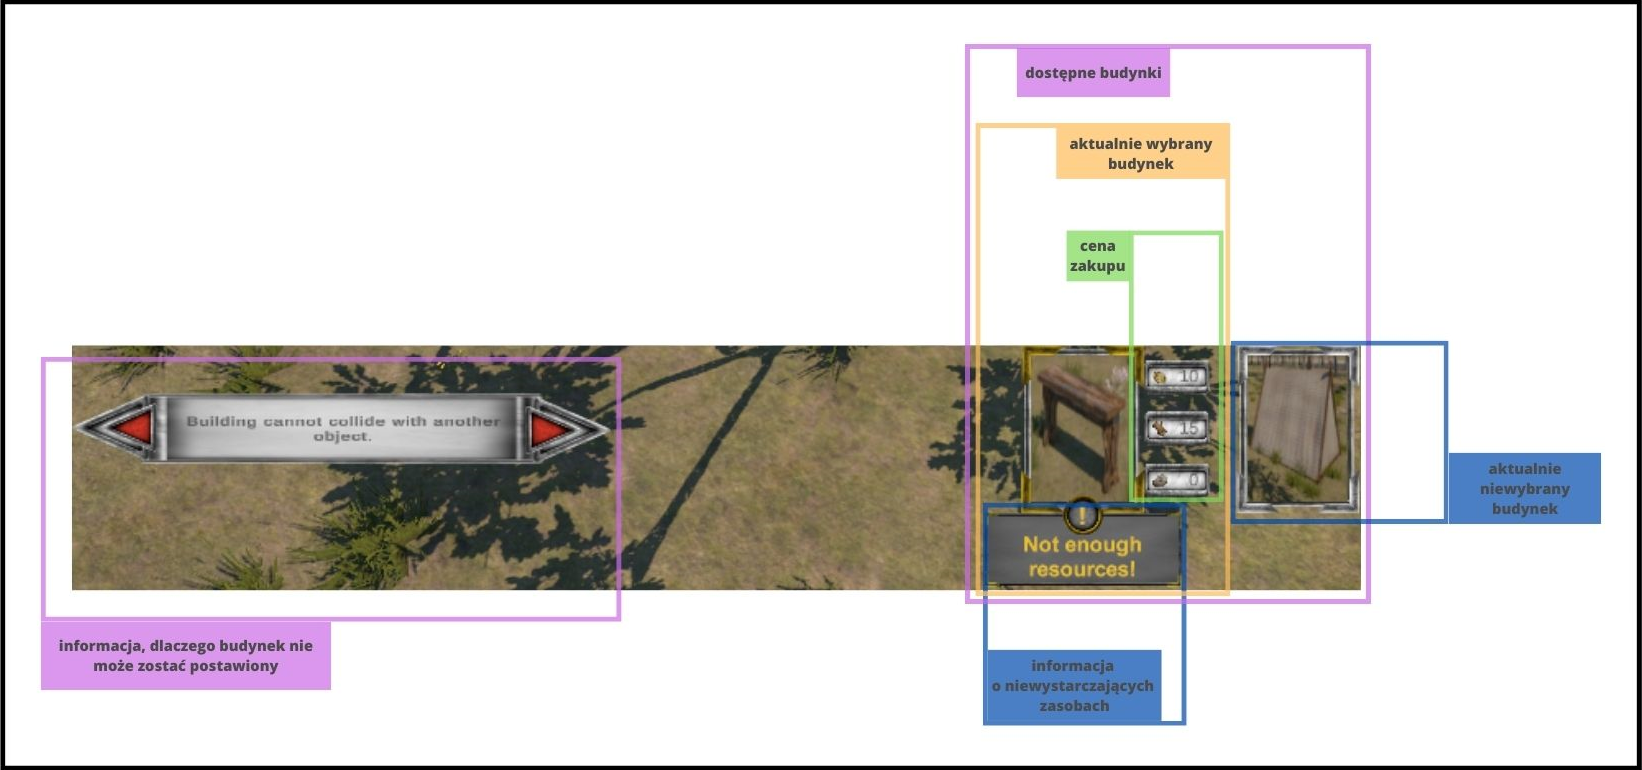
\includegraphics[width=0.9\textwidth]{images/ui/opis_ekementow_budowanie.png}
    \caption{Implementacja menu stawiania budynków, na którym pokazane są możliwe do zbudowania budowle 
    i szczegółowe informacje o ich dostępności.
    }\label{fig:compass}
\end{figure}

%\subsection{Tryb walki}%
